\documentclass[10pt]{article}
\usepackage{kotex}
\usepackage[margin=0.6in]{geometry} % set the margins to 1in on all sides
\usepackage{graphicx} % to include figures
\usepackage{amsmath} % great math stuff
\usepackage{amsfonts} % for blackboard bold, etc
\usepackage{amsthm} % better theorem environments
\usepackage{amssymb}
\usepackage[utf8]{inputenc}
\usepackage{booktabs}
\usepackage{array}
\usepackage{courier}
\usepackage[usenames, dvipsnames]{color}
\usepackage{titlesec}
\usepackage{empheq}
\usepackage{tikz}
\usepackage{wrapfig}
\usepackage{float}

\linespread{1.5}

\newcommand\encircle[1]{%
  \tikz[baseline=(X.base)] 
    \node (X) [draw, shape=circle, inner sep=0] {\strut #1};}
 
% Command "alignedbox{}{}" for a box within an align environment
% Source: http://www.latex-community.org/forum/viewtopic.php?f=46&t=8144
\newlength\dlf  % Define a new measure, dlf
\newcommand\alignedbox[2]{
% Argument #1 = before & if there were no box (lhs)
% Argument #2 = after & if there were no box (rhs)
&  % Alignment sign of the line
{
\settowidth\dlf{$\displaystyle #1$}  
    % The width of \dlf is the width of the lhs, with a displaystyle font
\addtolength\dlf{\fboxsep+\fboxrule}  
    % Add to it the distance to the box, and the width of the line of the box
\hspace{-\dlf}  
    % Move everything dlf units to the left, so that & #1 #2 is aligned under #1 & #2
\boxed{#1 #2}
    % Put a box around lhs and rhs
}
}


\newtheorem{thm}{Theorem}[section]
\newtheorem{lem}[thm]{Lemma}
\newtheorem{prop}[thm]{Proposition}
\newtheorem{cor}[thm]{Corollary}
\newtheorem{conj}[thm]{Conjecture}

\setcounter{secnumdepth}{4}

\titleformat{\paragraph}
{\normalfont\normalsize\bfseries}{\theparagraph}{1em}{}
\titlespacing*{\paragraph}
{0pt}{3.25ex plus 1ex minus .2ex}{1.5ex plus .2ex}

\definecolor{myblue}{RGB}{72, 165, 226}
\definecolor{myorange}{RGB}{222, 141, 8}

\setlength{\heavyrulewidth}{1.5pt}
\setlength{\abovetopsep}{4pt}


\DeclareMathOperator{\id}{id}
\DeclareMathOperator{\argmin}{\arg\!\min}
\DeclareMathOperator{\Tr}{Tr}

\newcommand{\bd}[1]{\mathbf{#1}} % for bolding symbols
\newcommand{\RR}{\mathbb{R}} % for Real numbers
\newcommand{\ZZ}{\mathbb{Z}} % for Integers
\newcommand{\col}[1]{\left[\begin{matrix} #1 \end{matrix} \right]}
\newcommand{\comb}[2]{\binom{#1^2 + #2^2}{#1+#2}}
\newcommand{\bs}{\boldsymbol}
\newcommand{\opn}{\operatorname}
\begin{document}
\nocite{*}

\title{$\pi$에 관하여}
\author{임대영 \\ 고려대학교 통계학과}
\maketitle

\section{$\pi$는 존재하지 않는다}
통계를 조금 공부해보면 다음과 같은 질문이 자주 생기게 된다. `실제로 정규 분포를 따르는 것이 있을까?' 통계 질문방에 가봐도 ``아이비리그에 들어가는 것은 확률과정인가요?'' 혹은 ``학생들의 성적은 정규분포인가요?''와 같은 질문이 수도 없이 많다. 이런 질문이 올라올 때마다 나의 답변은 ``이 세상에 존재하는 그 어떤 것도 확률과정이거나 정규분포를 따르는 것은 없습니다''이다. 수학을 공부하는 사람들이 가장 많이 하는 착각이 바로 이런 것이다. 수학 책에 나오는 모든 것들이 실재할 것이라는 착각. 물론 직관적으로 이해가 잘 되는 것은 있다. 자연수가 대표적이다. 이 때문에 레오폴트 크로네커(Leopold Kronecker)라는 과거 프로이센의 수학자는 다음과 같이 말하기도 했다.
\begin{center}
  ``정수는 신이 만들었지만 나머지는 인간의 창작물이다.'' (God made the integers. All else is the work of man.)
\end{center}
 `수'라는 것은 인간의 위대한 발명품이지만 실제로 존재하지는 않는다. 상당히 철학적이다. 숫자가 존재하지 않는다니! 하지만 잘 생각해보면 숫자라는 건 실재하는 것이 아니라 사람이 쓰기 좋게 만들어놓은 하나의 도구라는 것이 명료해질 것이다. 자꾸 이런 직관에 의존하려고 하다보니 어차피 다 실존하지 않는 창작물인데 유독 `허수'에만 허구라는 꼬리표를 달아놓는다. 하지만 허수를 포함한 복소수도 매우 직관적으로 이해할 수 있는 것들이며 그와 동시에 존재하지 않으면서도 많은 현상과 운동, 법칙을 설명할 수 있는 좋은 도구이다. 이러한 특성은 $\pi$라고 예외일 수 없다. 매우 충격적인 사실은 물리적인 형체를 지니고 있는 이 세상의 그 어떤 원도 원주와 지름의 비율이 정확히 $\pi$가 아니다. 모든 물리적인 측정에는 오차가 따른다. 다시 한 번 강조하지만 정확히 $\pi$의 값을 지니는 것은 없다. 있다고 해도 우리는 무엇이 `정확히' $\pi$의 값을 지니는지 알 턱이 없다. $\pi$는 없다.
\section{$\pi$가 원주율이 아니다}
\begin{wrapfigure}{r}{0.2\textwidth}
  \centering
  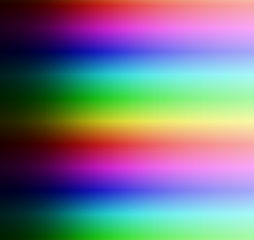
\includegraphics[width = 0.2\textwidth]{exp_mosaic.png}
  \caption{Mosaic image of $\exp\left(ix\right)$}
\end{wrapfigure}\par
$\pi$를 처음 배울 때 그 누구나 다 `원주율'이라고 배웠다. 반은 맞고 반은 틀렸다. 유클리드 기하에서는 원의 곡률이 0이고 원주와 지름의 비율이 $\pi$라는 상수가 된다. 하지만 쌍곡 기하에서는 곡률이 음수가 되며 원이 커지면 커질수록 원주와 지름의 비율은 무한대로 증가한다. 따라서 어떤 상수로 정의될 수 없다. 타원 기하에서도 마찬가지로 곡률이 양수이며 원주와 지름의 비율이 원이 커짐에 따라 감소한다. 여기서도 상수가 아니다. 그러면 $\pi$는 원주율이라고 정의할 때는 유클리드 기하를 전제하고 하는 말일 것이다. 무엇을 정의할 때 전제가 필요한 것과 전제가 필요없는 것이 있다면, 오컴의 법칙(Occam's razor)에 따라 전제가 필요없는 것을 따라야 할 터이다. 그렇다면 이러한 정의는 어떻게 할 수 있을까?\par
오른쪽에 있는 것은 복소지수함수의 모자이크 이미지이다. 패턴이 보이는가? 그렇다면 $\pi$의 흔적을 찾은 것이다. 조금 더 명확하게 보고 싶다면 아래의 그래프를 보자. 

% 한국에서 고등 교육을 받은 사람이라면 $\pi$를 모르는 사람은 없을 것이다. 하지만 매일 $\pi$를 써서 계산을 해 내는 물리학자나 수학자도 $\pi$에 대해 설명하라고 하면 단박에 그 정수를 찔러 설명하지 못할 듯싶다. 그토록 이 숫자에는 아주 중요한 성질이 있고 그것은 한 마디로 표현하기에는 너무 중요하다.\par
% $\pi$는 원주율이다. 분명 이 숫자는 원과 관련이 있다. 그러나 이러한 정의는 `틀렸다'고 할 수 있을 정도로 그 본질을 설명하지 못한다. $\pi$는 원이나 각도 따위를 알지 못한다. 예를 들어, 통계학에서 가장 중요한 정규 분포의 밀도 함수에 등장하는 $1/\sqrt{2\pi}$에서 원의 흔적을 발견할 수 있는가? 원의 성질과 연결시키지 않아도 우리는 충분히 정규 분포의 중요성을 설명할 수 있다. 왜냐하면 $\pi$는 원에서 나온 숫자가 아니기 때문이다. $\pi$는 원과 관련짓지 않고도 그 중요성을 명료하게 설명할 수 있는 숫자이다.\par
\begin{wrapfigure}{l}{0.5\textwidth}
  \centering
  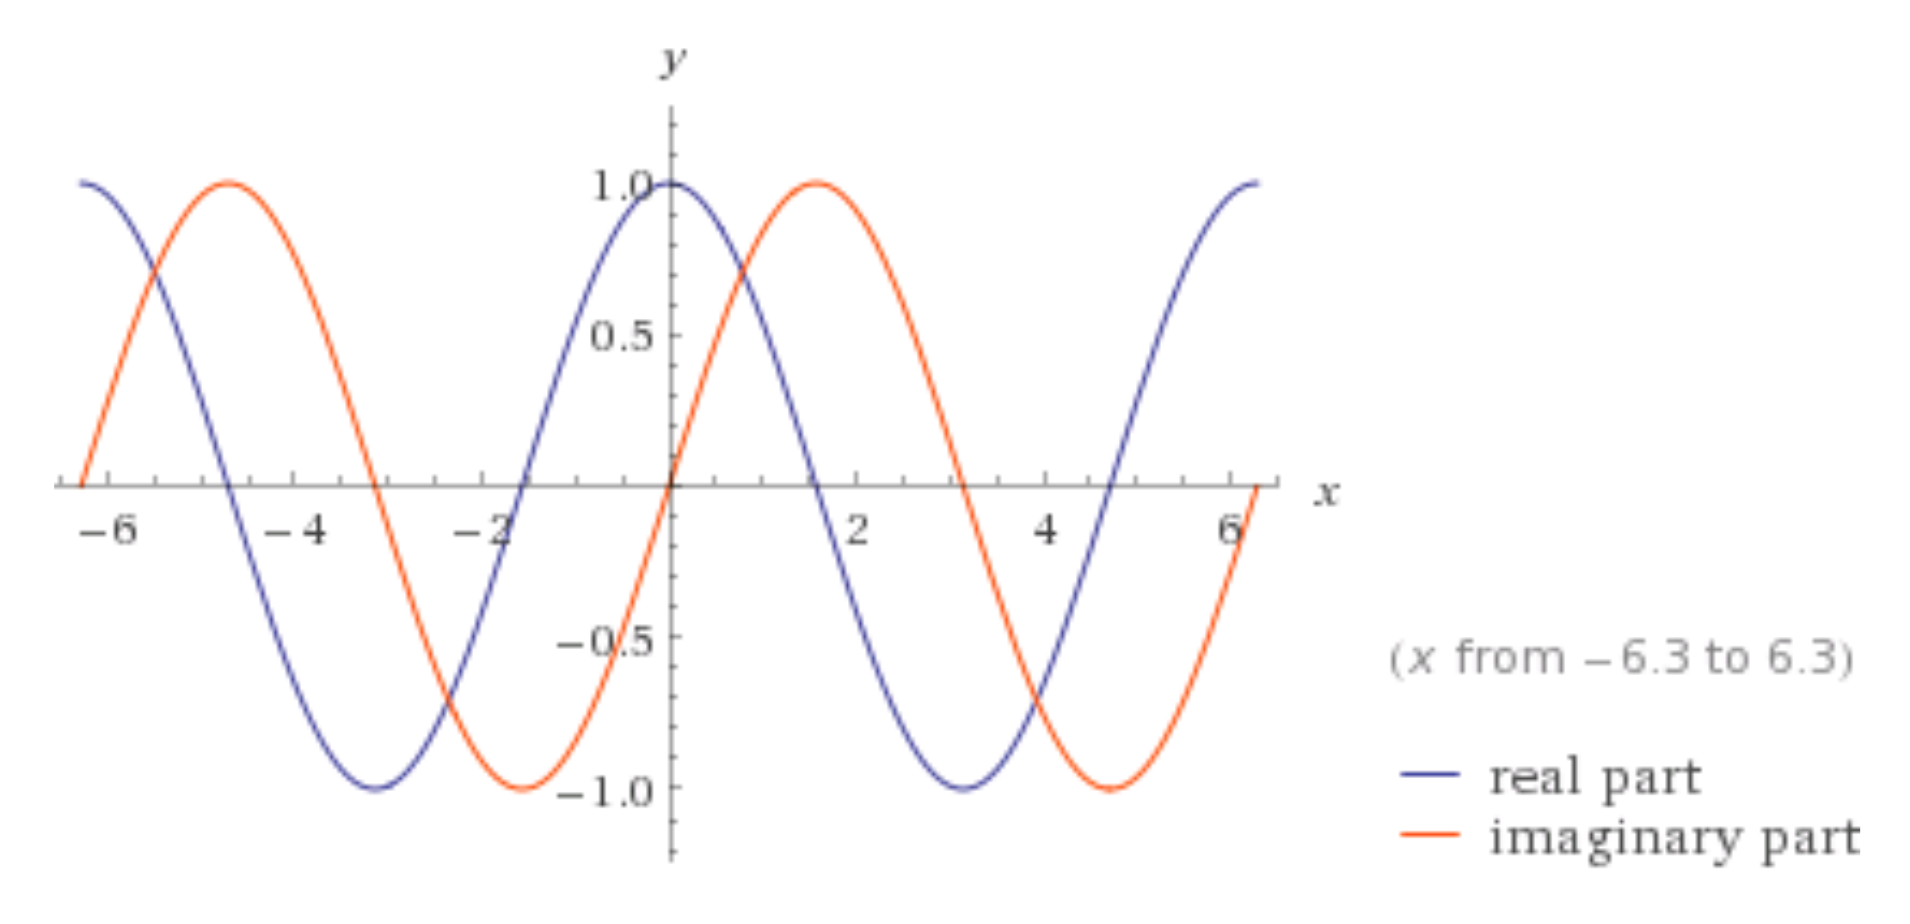
\includegraphics[width = 0.5\textwidth]{exponential.png}
  \caption{Graph of $\exp\left(ix\right)$}
\end{wrapfigure}
이 그래프에서 허수부가 움직이는 곡선을 잘 따라가다 보면 x축과의 교점이 3보다 약간 큰 수라는 것을 알 수 있다. 그리고 파동이 주기를 갖고 진동하고 있음을 볼 수 있다. 이 함수 하나가 $\pi$를 정의하면서도 그 중요성을 설명해 줄 수 있다. 왜 여기서 느닷없이 $\pi$가 등장하는 것일까? \par
이 모든 것의 근간에 있고 $\pi$와 $e$가 보편적으로 나타나는 그 원천에 있는 것이 다음의 간단하기 그지없는, 그렇지만 매우 강력하고도 중요한 방정식이다.
$$
  f' = f
$$

% 그렇다면 도대체 이 간단하고도 엄청나 보이는 숫자는 어떻게 해서 등장하게 된 것일까? 답은 바로 `지수 함수'에 있다. 복소 공간에서 지수 함수의 행적을 잘 살펴보면 $\pi$의 모습이 보일 것이다. 믿기지 않는가? 위의 그림을 보자. 이 그림은 $\exp\left(ix\right)$의 모자이크 이미지이다.
% 색깔이 반복되는 것을 보면 지수 함수가 어떠한 주기를 가지고 있음을 알 수 있다. 더 자세하게 보려면 복소 공간에서의 지수 함수를 실수부와 허수부를 따로 표현한 왼쪽의 그래프를 보아라. 예상했듯이 주기성을 보이고 있다. 지수 함수는 수학 문제를 풂에 있어서 도처에 나타나는데, 그 보편성은 다음의 미분방정식이 가장 기본이 모든 문제에서 가장 단순하고도 근간이 되기 때문이다.
% $$
%   f' = f
% $$
% 단순하기 그지없는 이 방정식이 만물의 움직임을 나타내는 미분 방적식의 기저에 깔려 있다니! 매우 놀라운 일이다. 이 방정식을 분석하다보면 자연스럽게 $\pi$와 $e$를 정의할 수 있게 된다. 

\end{document}


